\chapter{Results and Discussion}

The data and discussion of results below combine data gathered using the OONI probe in Ireland and Iraq with published OONI data from the OONI Measurement Aggregation Toolkit (MAT).

\section{Test Results}

\subsection{Website Accessibility Results}

\subsubsection{Collected Data}

This section analyses website accessibility data collected using the OONI Probe. The tests were carried out locally in Ireland and through a virtual machine (VM) hosted in Iraq. The results reflect the average number of websites blocked daily over a 9-day testing period. The findings are categorized by country, blocking method, and website category to highlight differences in censorship patterns.

\vspace{2em}

\begin{table}[H] 
\centering 
\caption{Proportion of Blocked vs. Unblocked Websites by Country (Daily Average Over 9 Days)} 
\begin{tabular}{lccc} 
\toprule 
\textbf{Country} & \textbf{Unblocked} & \textbf{Blocked} & \textbf{Blocked (\%)} \\
\midrule 
Ireland & 105 & 32 & 23.4\%  \\
Iraq & 108 & 29 & 21.2\% \\
\bottomrule 
\end{tabular} 
\label{tab:blocked_summary} 
\end{table}

It is worth noting that the results in table \ref{tab:blocked_summary} may not be reflective or indicator of the number of blocked websites in each country. The list of websites that yielded these results is comprised of commonly visited websites in each country along with some of the most known commonly blocked websites worldwide. A more in-depth discussion of these results can be found in section \ref{sec:Website-Accessability-Analysis}.

\vspace{2em}

\begin{table}[H] 
\centering 
\caption{Distribution of Detected Blocking Methods by Country} 
\begin{tabular}{lcccc} 
\toprule 
\textbf{Blocking Method} & \shortstack{\textbf{Iraq} \\ \textbf{Frequency}} & \textbf{Iraq \%} & \shortstack{\textbf{Ireland} \\ \textbf{Frequency}} & \textbf{Ireland \%} \\
\midrule 
TCP/IP         & 18 & 60.0\%  & 15 & 55.6\% \\
DNS            & 1  & 3.3\%   & 6  & 22.2\% \\
HTTP           & 3  & 10.0\%  & 1  & 3.7\% \\
Error/Failure  & 8  & 26.7\%  & 5  & 18.5\% \\
\bottomrule 
\end{tabular} 
\label{tab:blocking_methods_comparison} 
\end{table}

TCP/IP blocking emerged as the most common method, indicating low-level network interference. Ireland had more cases of DNS-based blocking than Iraq, whereas HTTP and Error/Failure blocks were more evenly distributed.

\vspace{2em}

\begin{table}[H] 
\centering 
\caption{Number of Blocked Websites by Category and Country} 
\begin{tabular}{lccc} 
\toprule 
\textbf{Category} & \textbf{Total} & \shortstack{\textbf{Ireland} \\ \textbf{Blocked (\%)}} & \shortstack{\textbf{Iraq} \\ \textbf{Blocked (\%)}} \\
\midrule 
Uncategorized                      & 30 & 12 (40.0\%)  & 10 (33.3\%) \\
Piracy / Streaming / File Sharing  & 20 & 10 (50.0\%)  & 4 (20.0\%)  \\
News / Media                       & 20 & 2 (10.0\%)   & 2 (10.0\%)  \\
Adult Content                      & 20 & 0 (0.0\%)    & 0 (0.0\%)   \\
Creative / Educational / Misc      & 15 & 0 (0.0\%)    & 0 (0.0\%)   \\
General / National Services        & 9  & 1 (11.1\%)   & 2 (22.2\%)  \\
Streaming / Social Media           & 9  & 1 (11.1\%)   & 1 (11.1\%)  \\
Religious                          & 4  & 2 (50.0\%)   & 3 (75.0\%)  \\
VoIP / Communication               & 2  & 1 (50.0\%)   & 1 (50.0\%)  \\
Gambling                           & 2  & 2 (100\%)    & 2 (100\%)   \\
Email/Privacy Tools                & 2  & 0 (0.0\%)    & 1 (50.0\%)  \\
Adult / Alcohol                    & 2  & 0 (0.0\%)    & 2 (100\%)   \\
LGBTQ+                             & 1  & 1 (100\%)    & 1 (100\%)   \\
AI / Technology                    & 1  & 0 (0.0\%)    & 0 (0.0\%)   \\
\bottomrule 
\end{tabular} 
\label{tab:category_block} 
\end{table}

The most frequently blocked category in Ireland was “Piracy / Streaming / File Sharing” (50\%), followed closely by “Uncategorized” sites (40\%). In Iraq, “Religious” websites experienced the highest rate of censorship (75\%), with additional blocks targeting sites associated with adult content and gambling.

\subsubsection{Public OONI Data}

This section is an analysis of publicly available OONI data over the previous 30 day period in Ireland and Iraq. The data in table \ref{tab:category_block} is the average over the 30-day period.

\vspace{2em}

\begin{table}[H]
\centering
\caption{Website Blocking based on Public OONI Data}
\begin{tabular}{lcc}
\toprule
\textbf{} & \textbf{Ireland} & \textbf{Iraq} \\
\midrule
Number of Websites Tested           & 1695 & 3703 \\
Number of Successful Connections    & 1628 & 3353 \\
Number of Anomalies                 & 43 & 262 \\
Number of Failures                  & 24 & 88 \\
\bottomrule
Percentage of Total Blocked         & 2.5\% & 7\% \\
\end{tabular}
\label{tab:category_block}
\end{table}

\begin{figure}[H]
    \centering
    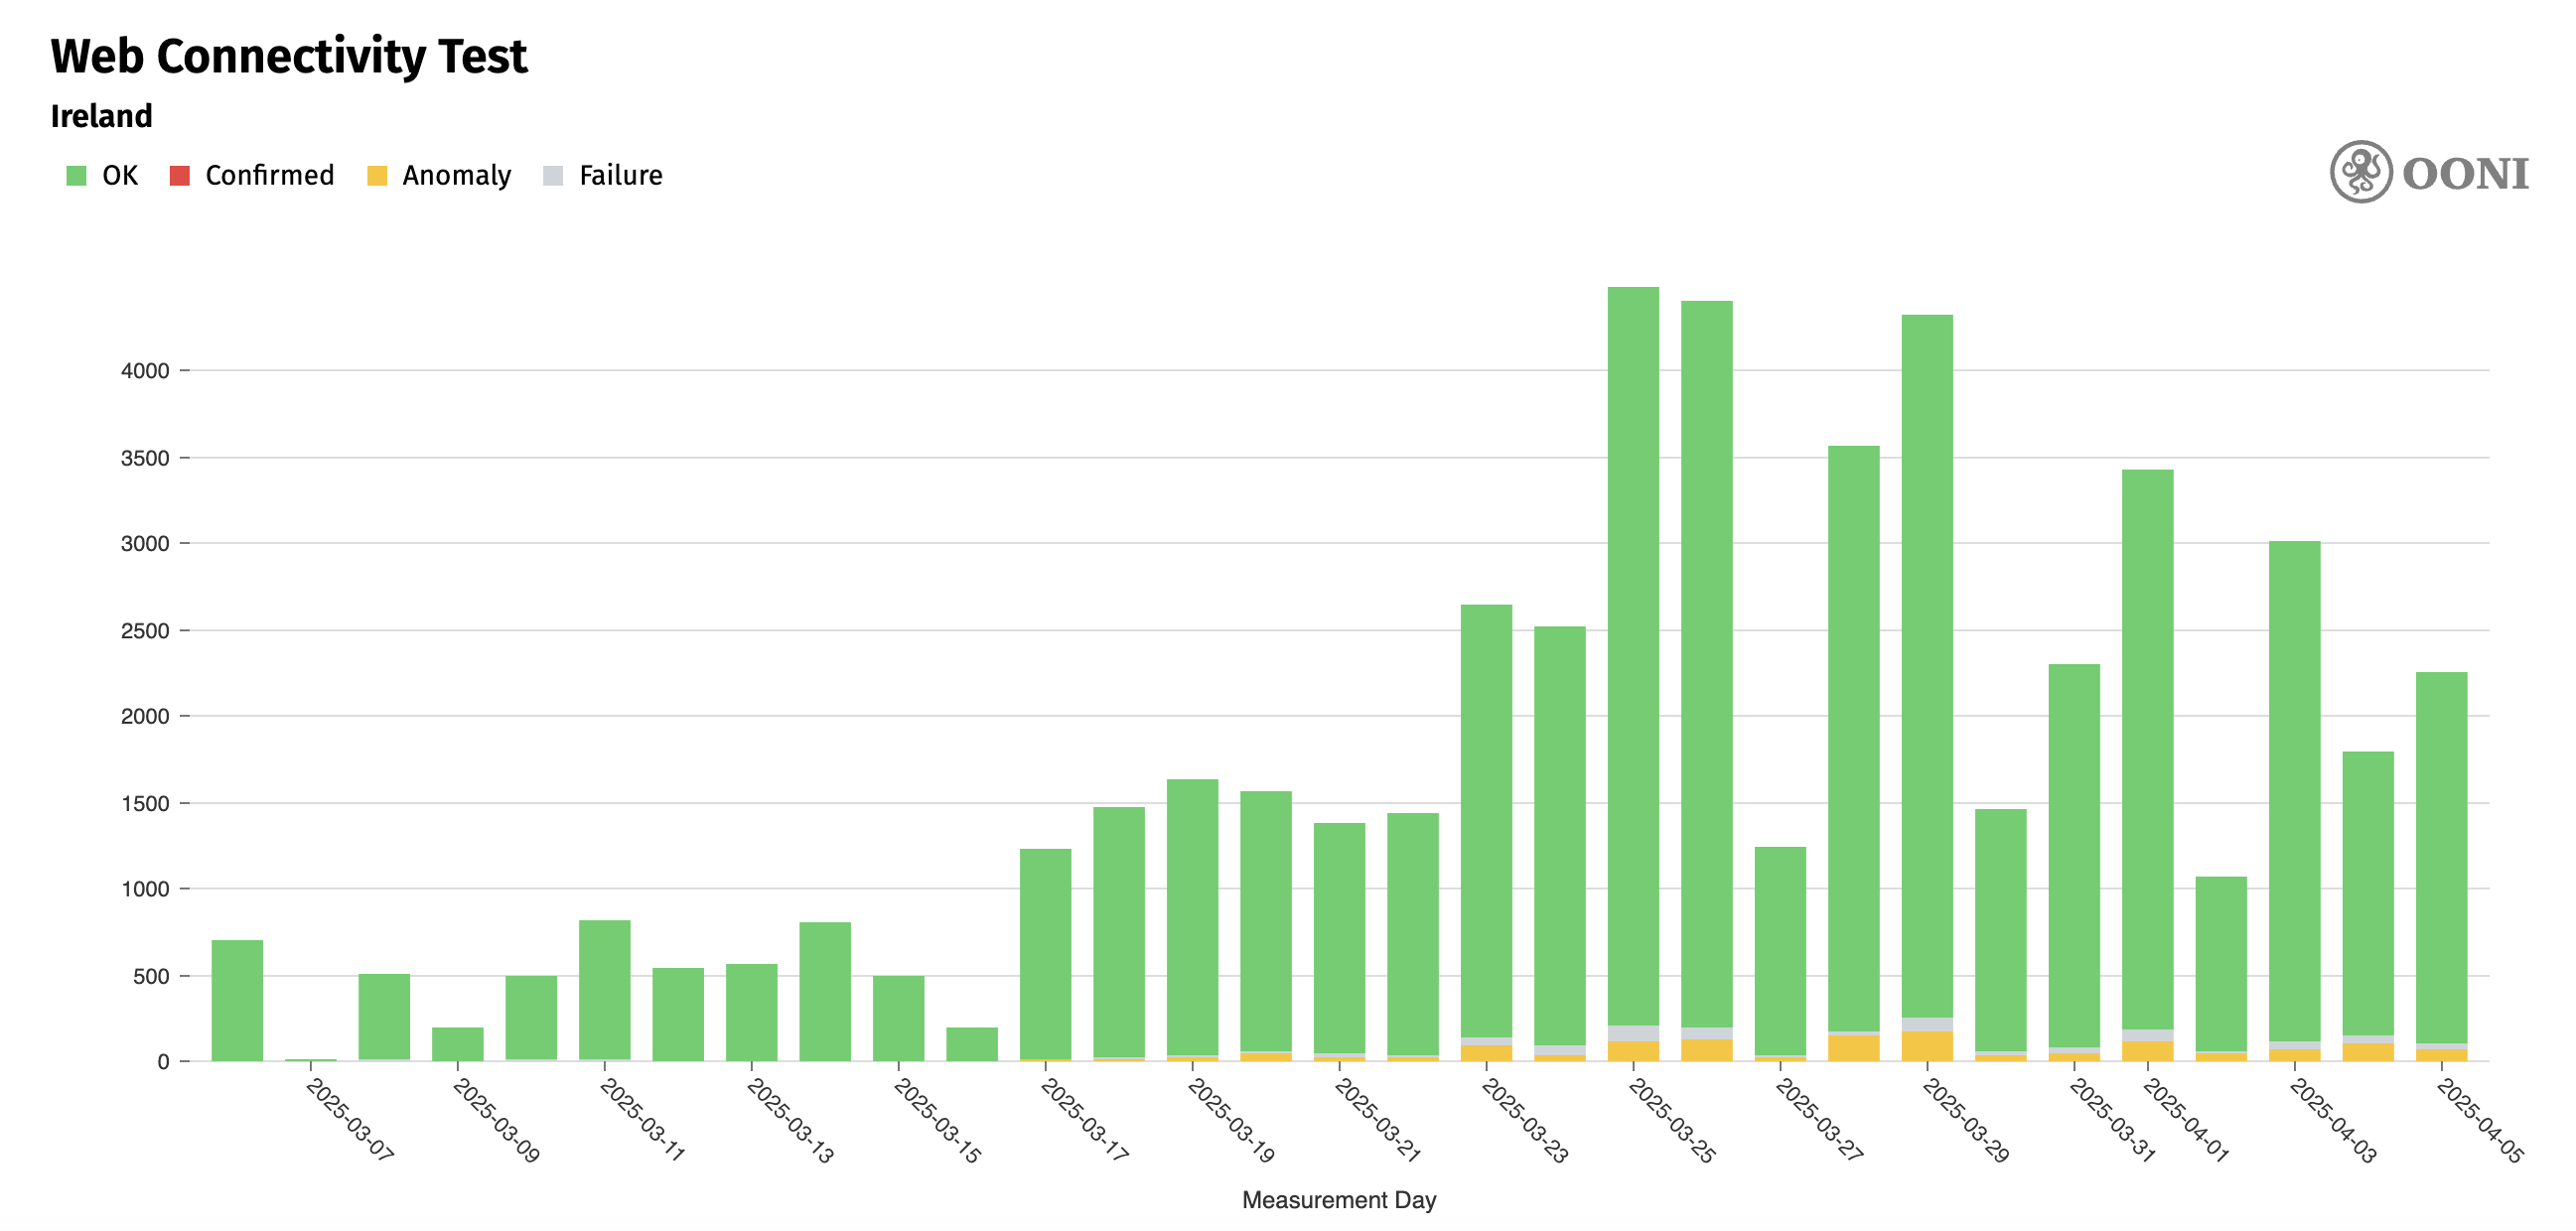
\includegraphics[width=\textwidth]{Griff/TCD SCSS CAPSTONE/Results/IrelandWebsiteTest.png}
    \caption{Ireland Web Connectivity Test: March 6, 2025 -- April 6, 2025}
    \label{fig:iraq-middlebox-HTTP-manipulation}
\end{figure}

\begin{figure}[H]
    \centering
    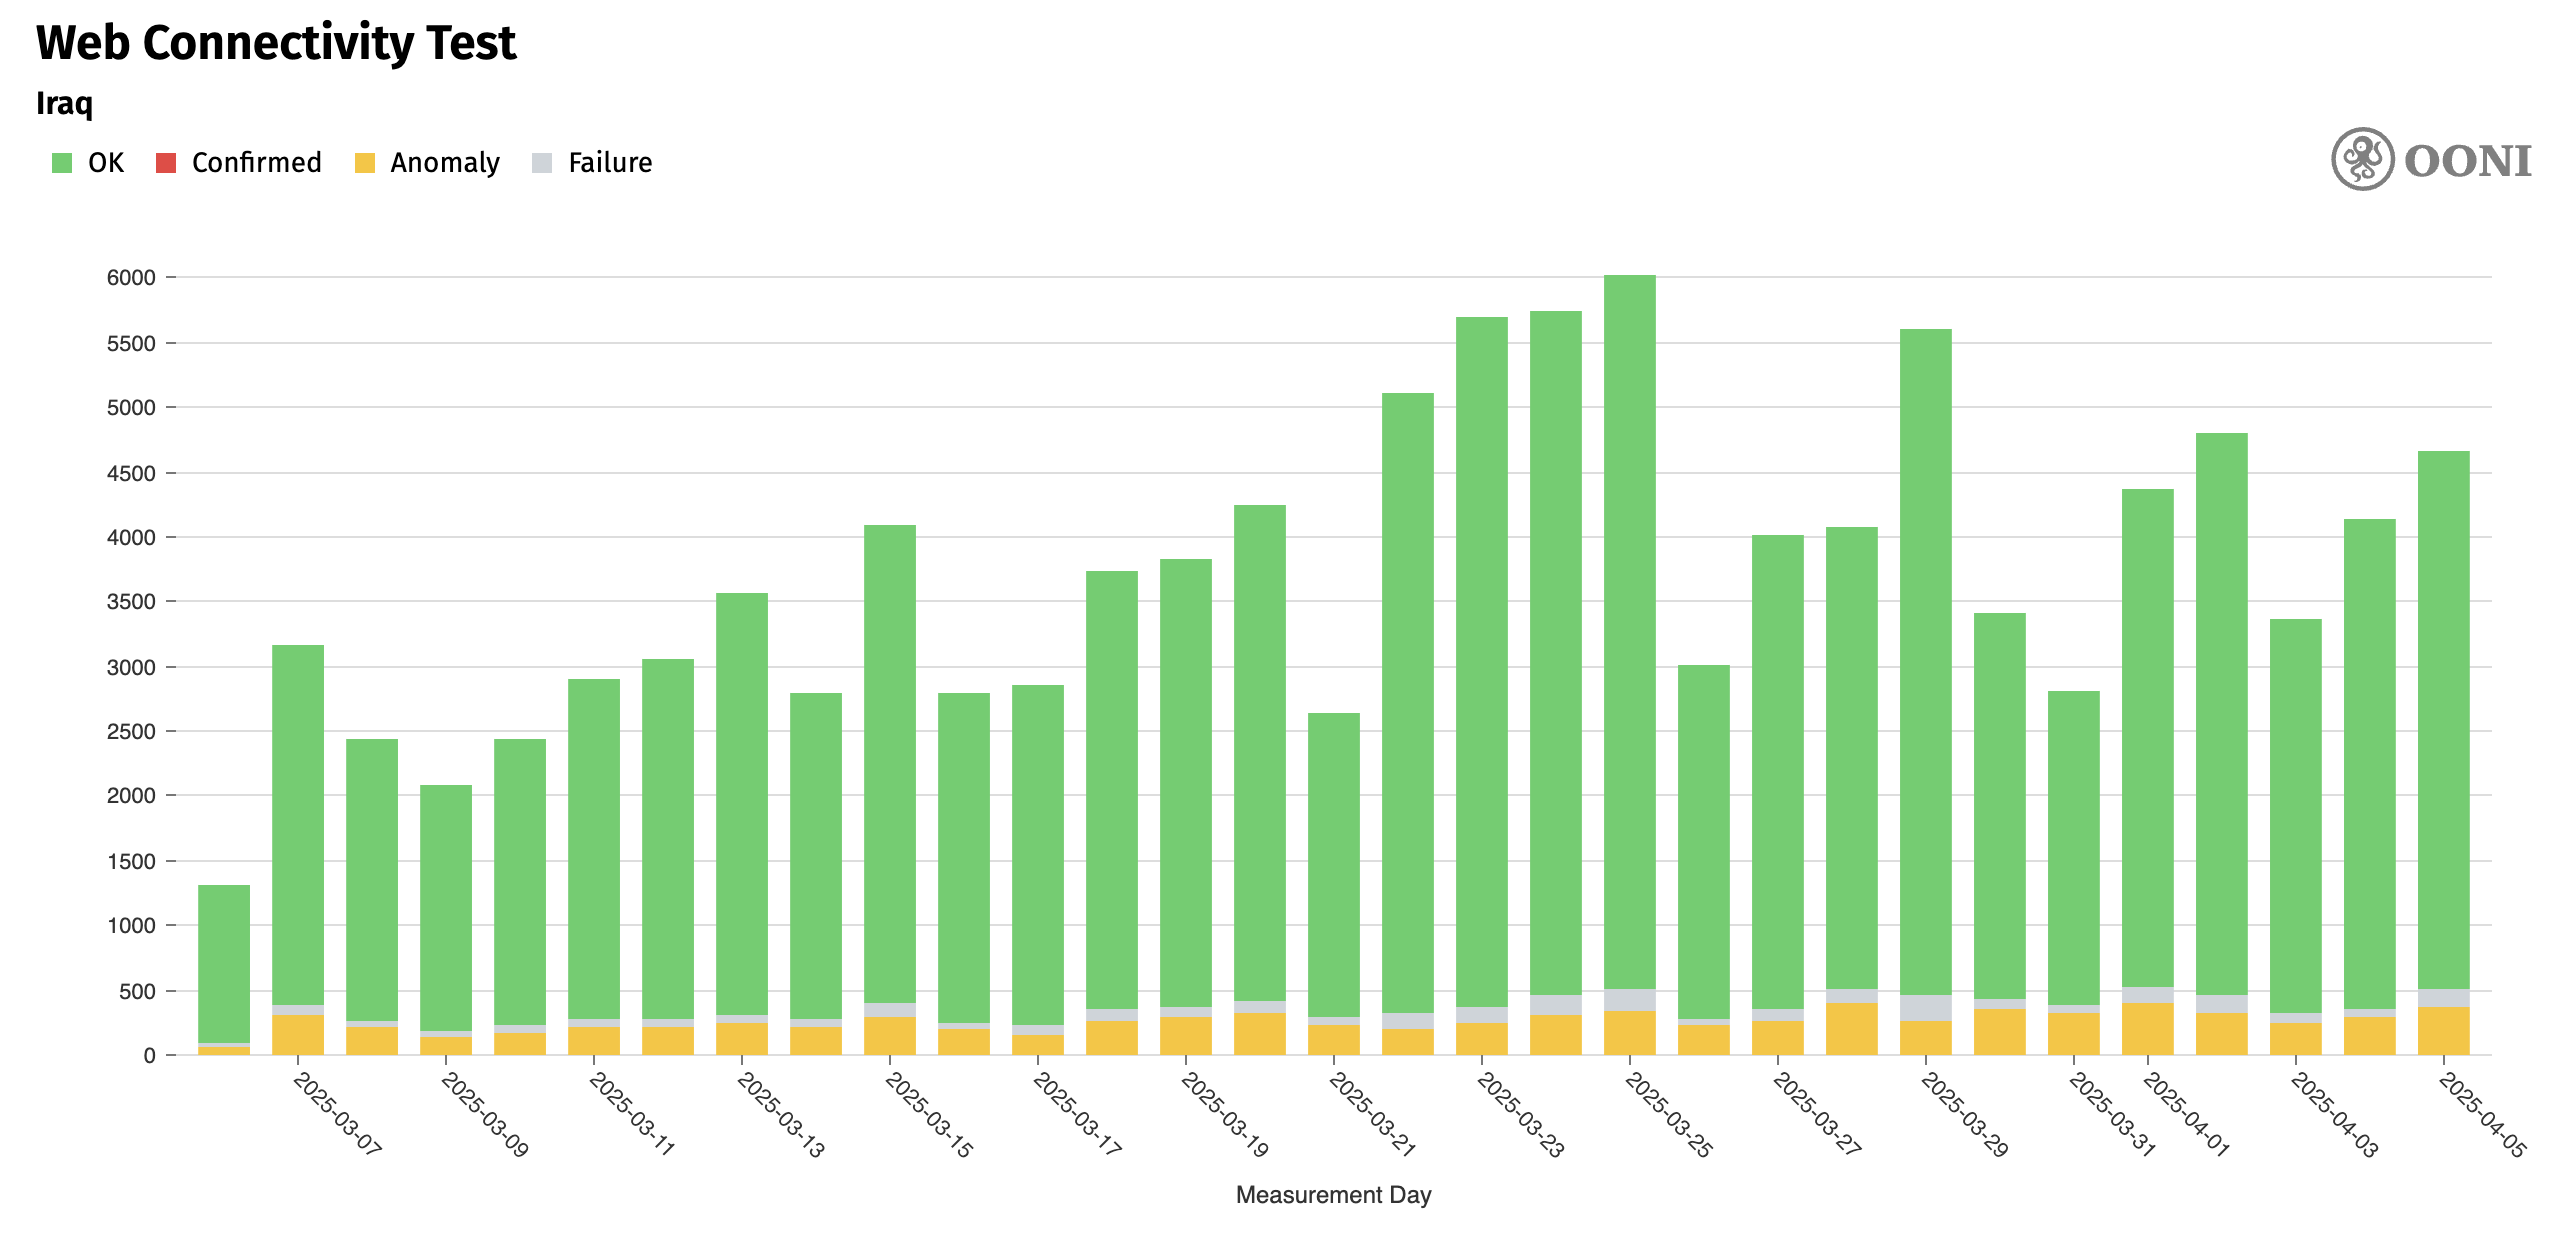
\includegraphics[width=\textwidth]{Griff/TCD SCSS CAPSTONE/Results/IraqWebsiteTest.png}
    \caption{Iraq Web Connectivity Test: March 6, 2025 -- April 6, 2025}
    \label{fig:iraq-middlebox-HTTP-manipulation}
\end{figure}

\subsection{Circumvention Test Results}

\subsubsection{Ireland}

Ireland likely does not block Tor on any ASNs, as it is largely accessible outside two anomalies.

\textbf{March 18, 2025} - Magnet Networks Limited (AS34245) - Tor Test (1 anomaly out of 78 measurements)
%https://explorer.ooni.org/m/20250318181530.182975_IE_tor_8b558463294b2881

\textbf{March 31, 2025} - Liberty Global B.V. (AS6830) - Tor Test (1 anomaly out of 191 measurements)
%https://explorer.ooni.org/m/20250331102020.562562_IE_tor_913ee551111fe0a9

Outside of these two anomalies, there is no evidence that Tor is being blocked in Ireland.

Psiphon, on the other hand, yielded different results. While Psiphon was largely able to be accessed on most ASNs, there were a few where access was likely blocked. 

\vspace{2em}

\begin{table}[H]
\centering
\caption{Networks in Ireland with Evidence of Psiphon Blocking}
\begin{tabular}{lccccc}
\toprule
\textbf{Network Name} & \textbf{ASN} & \shortstack{\textbf{Psiphon} \\ \textbf{Blocking Events}} & \shortstack{\textbf{Total} \\ \textbf{Measurements}} & \shortstack{\textbf{Block} \\ \textbf{Rate (\%)}} \\
\midrule
Microsoft Corporation           & AS8075  & 1  & 1   & 100\%  \\
HEAnet Ltd.                     & AS1213  & 33 & 35  & 94\%   \\
O2 Ireland Ltd.                 & AS13280 & 8  & 12  & 66\%   \\
Vodafone Ireland Ltd.           & AS15751 & 1  & 9   & 11\%   \\
Liberty Global B.V.             & AS6830  & 16 & 215 & 7.4\%  \\
\bottomrule
\textbf{Total} &  & \textbf{59} & \textbf{494} & \textbf{12.1\%} \\
\end{tabular}

\vspace{1em}

\caption*{\textit{Note:} "Psiphon Blocking Events" represent detected anomalies during testing of the Psiphon circumvention tool. "Block Rate" indicates the percentage of measurements that showed blocking behavior.}
\label{tab:psiphon_block_ireland}
\end{table}

\subsubsection{Iraq}

Like Ireland, Iraq does not block access to Tor, except for a few outliers.

\textbf{March 20, 2025} - Super Cell Network for Internet Services LTD (AS209193) - Tor Test (1 anomaly out of 92 measurements)
%https://explorer.ooni.org/m/20250320220102.873661_IQ_tor_3796e6aaa913670d

\textbf{March 30, 2025} - Hulum Almustakbal Company for Communication Engineering and Services Ltd (AS203214) - Tor Test (2 anomalies out of 160 measurements)
%https://explorer.ooni.org/m/20250330191838.341920_IQ_tor_f0e7ccd345c39d7f

\textbf{March 30, 2025} - Valin Company for General Trading and Communications LTD (AS205254) - Tor Test (1 anomaly out of 17 measurements)
%https://explorer.ooni.org/m/20250330111106.914884_IQ_tor_f45745fcedc21407

Outside of these anomalies, no significant evidence exists that Tor is being blocked in Iraq.

There is also little evidence of Psiphon being blocked in Iraq significantly. Aside from a few outliers, Psiphon only seemed to be blocked on one ASN. 

\vspace{2em}

\begin{table}[H]
\centering
\caption{Networks in Iraq with Evidence of Psiphon Blocking}
\begin{tabular}{lccccc}
\toprule
\textbf{Network Name} & \textbf{ASN} & \shortstack{\textbf{Psiphon} \\ \textbf{Blocking Events}} & \shortstack{\textbf{Total} \\ \textbf{Measurements}} & \shortstack{\textbf{Block} \\ \textbf{Rate (\%)}} \\
\midrule
HulumTele             & AS203214  & 127 & 165  & 77\%   \\
NB Telecom            & AS208324  & 1   & 3    & 33\%   \\
AsiaCell Telecom      & AS51684   & 4   & 23   & 17\%   \\
Valin Co LTD          & AS205254  & 1   & 30   & 3.3\%  \\
Earthlink Telecom     & AS199739  & 1   & 352  & 0.2\%  \\
\bottomrule
\textbf{Total}        &           & \textbf{134} & \textbf{1107} & \textbf{12.1\%} \\
\end{tabular}

\vspace{1em}

\caption*{\textit{Note:} "Psiphon Blocking Events" refer to instances where the Psiphon circumvention tool exhibited signs of interference. "Block Rate" is calculated as the percentage of blocked measurements over the total measured on each network.}
\label{tab:psiphon_block_iraq}
\end{table}

\subsection{Instant Messaging Test Results}

The results of the Instant Messaging tests were very similar in Ireland and Iraq. Both tests showed no signs of interference or blocking of Facebook Messenger, Telegram, Whatsapp, or Signal. However, looking outside the tested ASNs reveals a significant difference between the two countries. The tested data in Ireland is consistent with public OONI data and shows no blocking of instant messaging platforms. The Iraq data is also consistent with tests run on the same ASN, but in Iraq, other ASNs show signs of blocking.

\subsubsection{Ireland}

In the past 30-day period, there were only 2 anomalies found that shows any kind of instant messaging blocking:

\textbf{March 24, 2025} - Packethub S.A. (AS136787) - Facebook Messenger Test (1 anomaly out of 3 measurements)
%https://explorer.ooni.org/m/20250324111124.418686_IE_facebookmessenger_fbdc8895400acaba

\textbf{March 24, 2025} - HEAnetCLG (AS1213) - Signal Test (1 anomaly out of 37 measurements)
%https://explorer.ooni.org/m/20250324164458.153631_IE_signal_667f7ad13e55043a

Outside of these anomalies, there was no evidence of instant messaging blocking.

\subsubsection{Iraq}

Iraq had significant evidence of instant messaging platforms being blocked in certain ASNs. The table below shows each ASN and the percentage of tests where an anomaly was found.

\vspace{2em}

\begin{table}[H]
\centering
\caption{Networks in Iraq with Evidence of Instant Messaging Platform Blocking}
\begin{tabular}{lcccccc}
\toprule
\textbf{Network Name} & \textbf{ASN} & \shortstack{\textbf{Facebook} \\ \textbf{Block Rate}} & \shortstack{\textbf{Telegram} \\ \textbf{Block Rate}} & \shortstack{\textbf{WhatsApp} \\ \textbf{Block Rate}} & \shortstack{\textbf{Signal} \\ \textbf{Block Rate}} \\
\midrule
CIT Co LTD            & AS212330  & 100\% & 0\%   & 0\%   & 0\%   \\
KNET                  & AS206206  & 60\%  & 0\%   & 0\%   & 0\%   \\
Cloudflare, Inc.      & AS13335   & 47\%  & 0\%   & 0\%   & 0\%   \\
Earthlink Telecom     & AS50710   & 33\%  & 0\%   & 0\%   & 0\%   \\
HulumTele             & AS203214  & 27\%  & 7.8\% & 25\%  & 44\%  \\
Valin Co LTD          & AS205254  & 26\%  & 3.8\% & 7.6\% & 7.6\% \\
Al-Nazeera Co.        & AS51020   & 0\%   & 0\%   & 0\%   & 32\%  \\
Noor Al-Bedaya Co.    & AS202651  & 0\%   & 0\%   & 0\%   & 23\%  \\
TLLG Co.              & AS210022  & 0\%   & 0\%   & 0\%   & 82\%  \\
Al Atheer Co. LTD     & AS59588   & 0\%   & 0\%   & 1.9\% & 1.9\% \\
Earthlink Telecom     & AS199739  & 1\%   & 0.5\% & 0.2\% & 0.8\% \\
Super Cell            & AS209193  & 0\%   & 0\%   & 0.7\% & 0\%   \\
\bottomrule
\textbf{Total Block Rate} & & \textbf{6.2\%} & \textbf{1.4\%} & \textbf{4.1\%} & \textbf{6.2\%} \\
\end{tabular}

\vspace{1em}

\caption*{\textit{Note:} Each percentage reflects the proportion of measurements on the respective network where blocking behavior was detected for a specific instant messaging platform. The platforms analyzed include Facebook Messenger, Telegram, WhatsApp, and Signal.}
\label{tab:im_block_iraq}
\end{table}

\subsection{Middlebox Test Results}

The results of the Middlebox Test were the same for both countries. Both the HTTP Header Field Manipulation and HTTP Invalid Request Line tests detected no Middleboxes in either country. However, while there was no evidence of Middleboxes being found using the providers tested, it is possible that other providers in both countries have Middleboxes present in the network.

Using publicly available OONI data for Ireland and Iraq, it was found that Middleboxes were detected in both countries over the past 30 days (March 6, 2025 - April 6, 2025). 

\subsubsection{Ireland}

There is very little evidence of Middleboxes in Ireland. Over the past 30-day period, only two anomalies have been present. Both of these anomalies are from the HTTP Invalid Request Line test. 

\textbf{March 25, 2025} - Meteor Mobile Communications Ireland (AS15751) (1 anomaly out of 9 measurements)
%https://explorer.ooni.org/m/20250325122211.663367_IE_httpinvalidrequestline_c713442d98eebb5c

\textbf{April 1, 2025} - Vodafone Ireland Limited (AS15502) (1 anomaly out of 79 measurements)
%https://explorer.ooni.org/m/20250401215651.365763_IE_httpinvalidrequestline_51f20fe7e9d31698

These results are likely outliers, as there were very few Middlebox tests for Meteor Mobile Communications Ireland during this time span and no other anomalies for Vodafone Ireland Limited.

\subsubsection{Iraq}

There is considerably more evidence of Middleboxes in Iraq. Over the past 30 days, there were 125 anomalies in the HTTP Invalid Request line Test and 19 anomalies in the HTTP Header Field Manipulation Test.

The table below lists the ASNs suspected to have Middleboxes present using the HTTP Invalid Request Line test. It then shows the number of anomalies, the total measurement count, and the percentage of the total count that was anomalies.

\vspace{2em}

\begin{table}[H]
\centering
\caption{Networks in Iraq with Evidence of Middleboxes (HTTP Invalid Request Line Test)}
\begin{tabular}{lccccc}
\toprule
\textbf{Network Name} & \textbf{ASN} & \shortstack{\textbf{Detected} \\ \textbf{Events}} & \shortstack{\textbf{Total} \\ \textbf{Measurements}} & \shortstack{\textbf{Block} \\ \textbf{Rate (\%)}} \\
\midrule
EarthLink Ltd.        & AS50710   & 1  & 1   & 100\%    \\
Al-Jazeera Co.        & AS198589  & 68 & 70  & 97\%     \\
Cloudflare, Inc.      & AS13335   & 8  & 10  & 80\%     \\
IQ-Online             & AS48492   & 2  & 4   & 50\%     \\
Al Atheer Co. LTD     & AS59588   & 13 & 53  & 24.5\%   \\
HulumTele             & AS203214  & 32 & 158 & 20.25\%  \\
\bottomrule
\textbf{Total} & & \textbf{125} & \textbf{1071} & \textbf{11.6\%} \\
\end{tabular}

\vspace{1em}

\caption*{\textit{Note:} This table presents results from the HTTP Invalid Request Line Test. "Detected Events" refer to anomalies suggesting the presence of network middleboxes. "Block Rate" is the percentage of such events relative to the total measurements per ASN.}
\label{tab:middlebox_http_invalid}
\end{table}

%\begin{figure}[H]
%    \centering
%    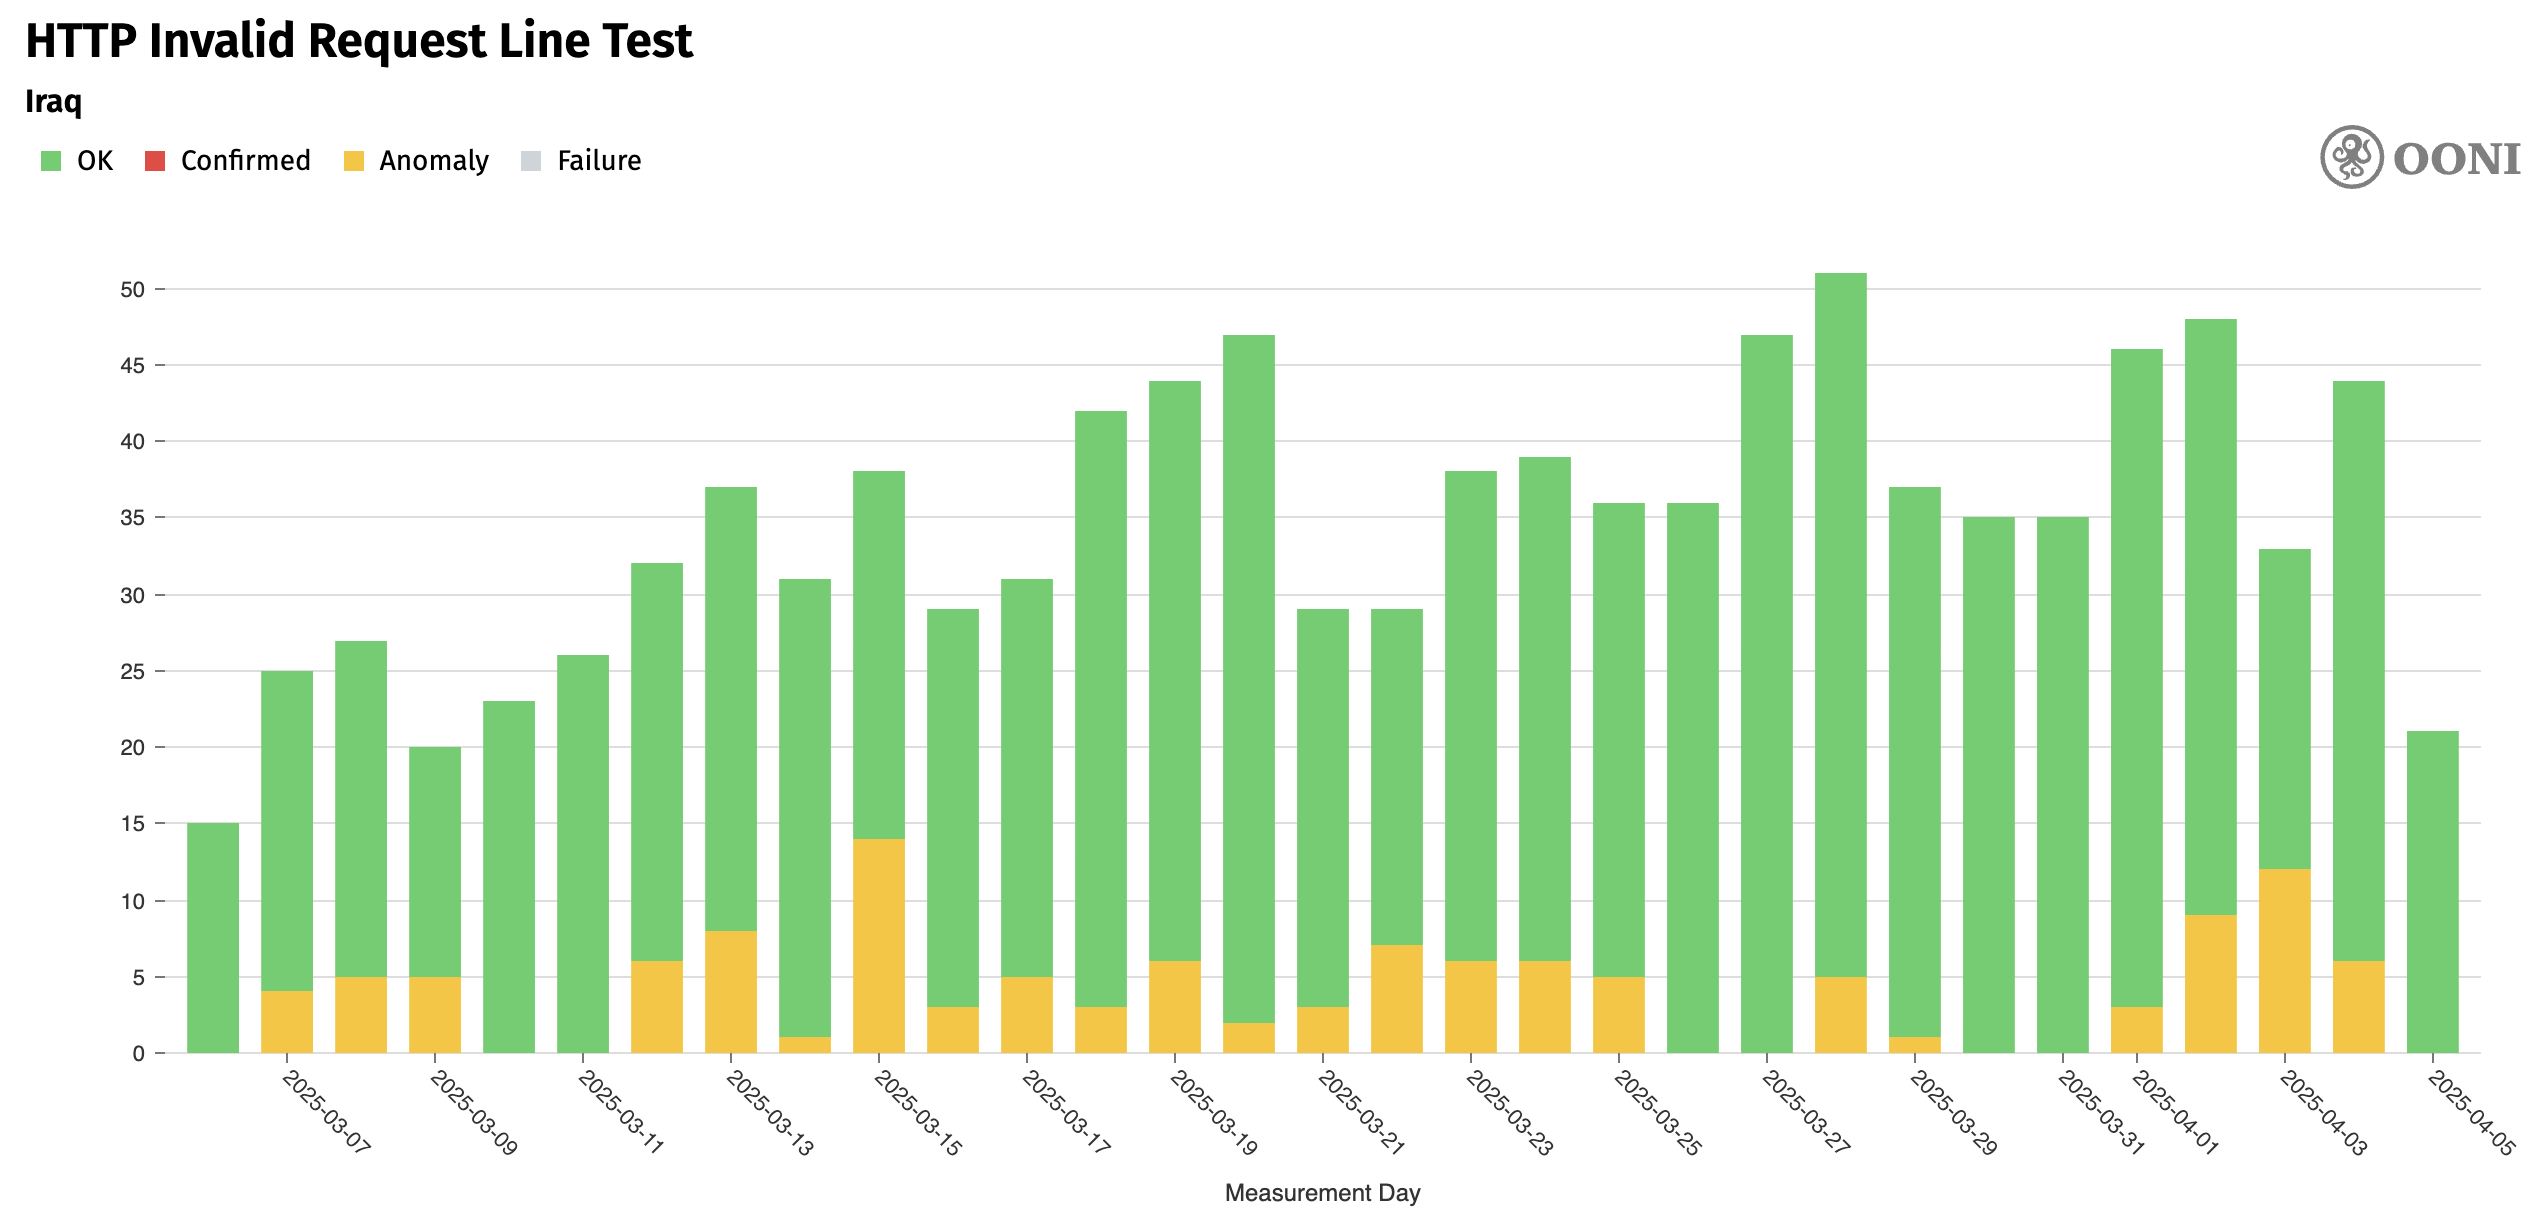
\includegraphics[width=\textwidth]{Griff/TCD SCSS CAPSTONE/Results/IraqMiddleboxHTTPInvalidTest.png}
 %   \caption{Iraq Middlebox HTTP Invalid Request Line Test: March 6, 2025 -- April 6, 2025}
%    \label{fig:iraq-middlebox-invalid-request}
%\end{figure}

The table below lists the ASNs suspected to have Middleboxes present using the HTTP Header Field Manipulation test. It then shows the number of anomalies, the total measurement count, and what percentage of the total count were anomalies. Note that any ASN that had less than 0.5\% anomalies was ignored.

\vspace{2em}

\begin{table}[H]
\centering
\caption{Networks in Iraq with Evidence of Middleboxes (HTTP Header Field Manipulation Test)}
\begin{tabular}{lccccc}
\toprule
\textbf{Network Name} & \textbf{ASN} & \shortstack{\textbf{Detected} \\ \textbf{Events}} & \shortstack{\textbf{Total} \\ \textbf{Measurements}} & \shortstack{\textbf{Block} \\ \textbf{Rate (\%)}} \\
\midrule
EarthLink Ltd.        & AS50710  & 1 & 1  & 100\%  \\
Cloudflare, Inc.      & AS13335  & 8 & 10 & 80\%   \\
IQ-Online             & AS48492  & 2 & 4  & 50\%   \\
\bottomrule
\textbf{Total} & & \textbf{11} & \textbf{15} & \textbf{1.7\% of full dataset (1074)} \\
\end{tabular}

\vspace{1em}

\begin{minipage}{0.95\linewidth}
\caption*{\textit{Note:} This test detects potential middleboxes by observing anomalies in how HTTP header fields are processed. "Detected Events" are instances of irregular responses, possibly caused by network interference. "Block Rate" indicates the ratio of these events to total measurements per ASN.}
\end{minipage}
\label{tab:middlebox_http_header}
\end{table}

%\begin{figure}[H]
 %   \centering
%    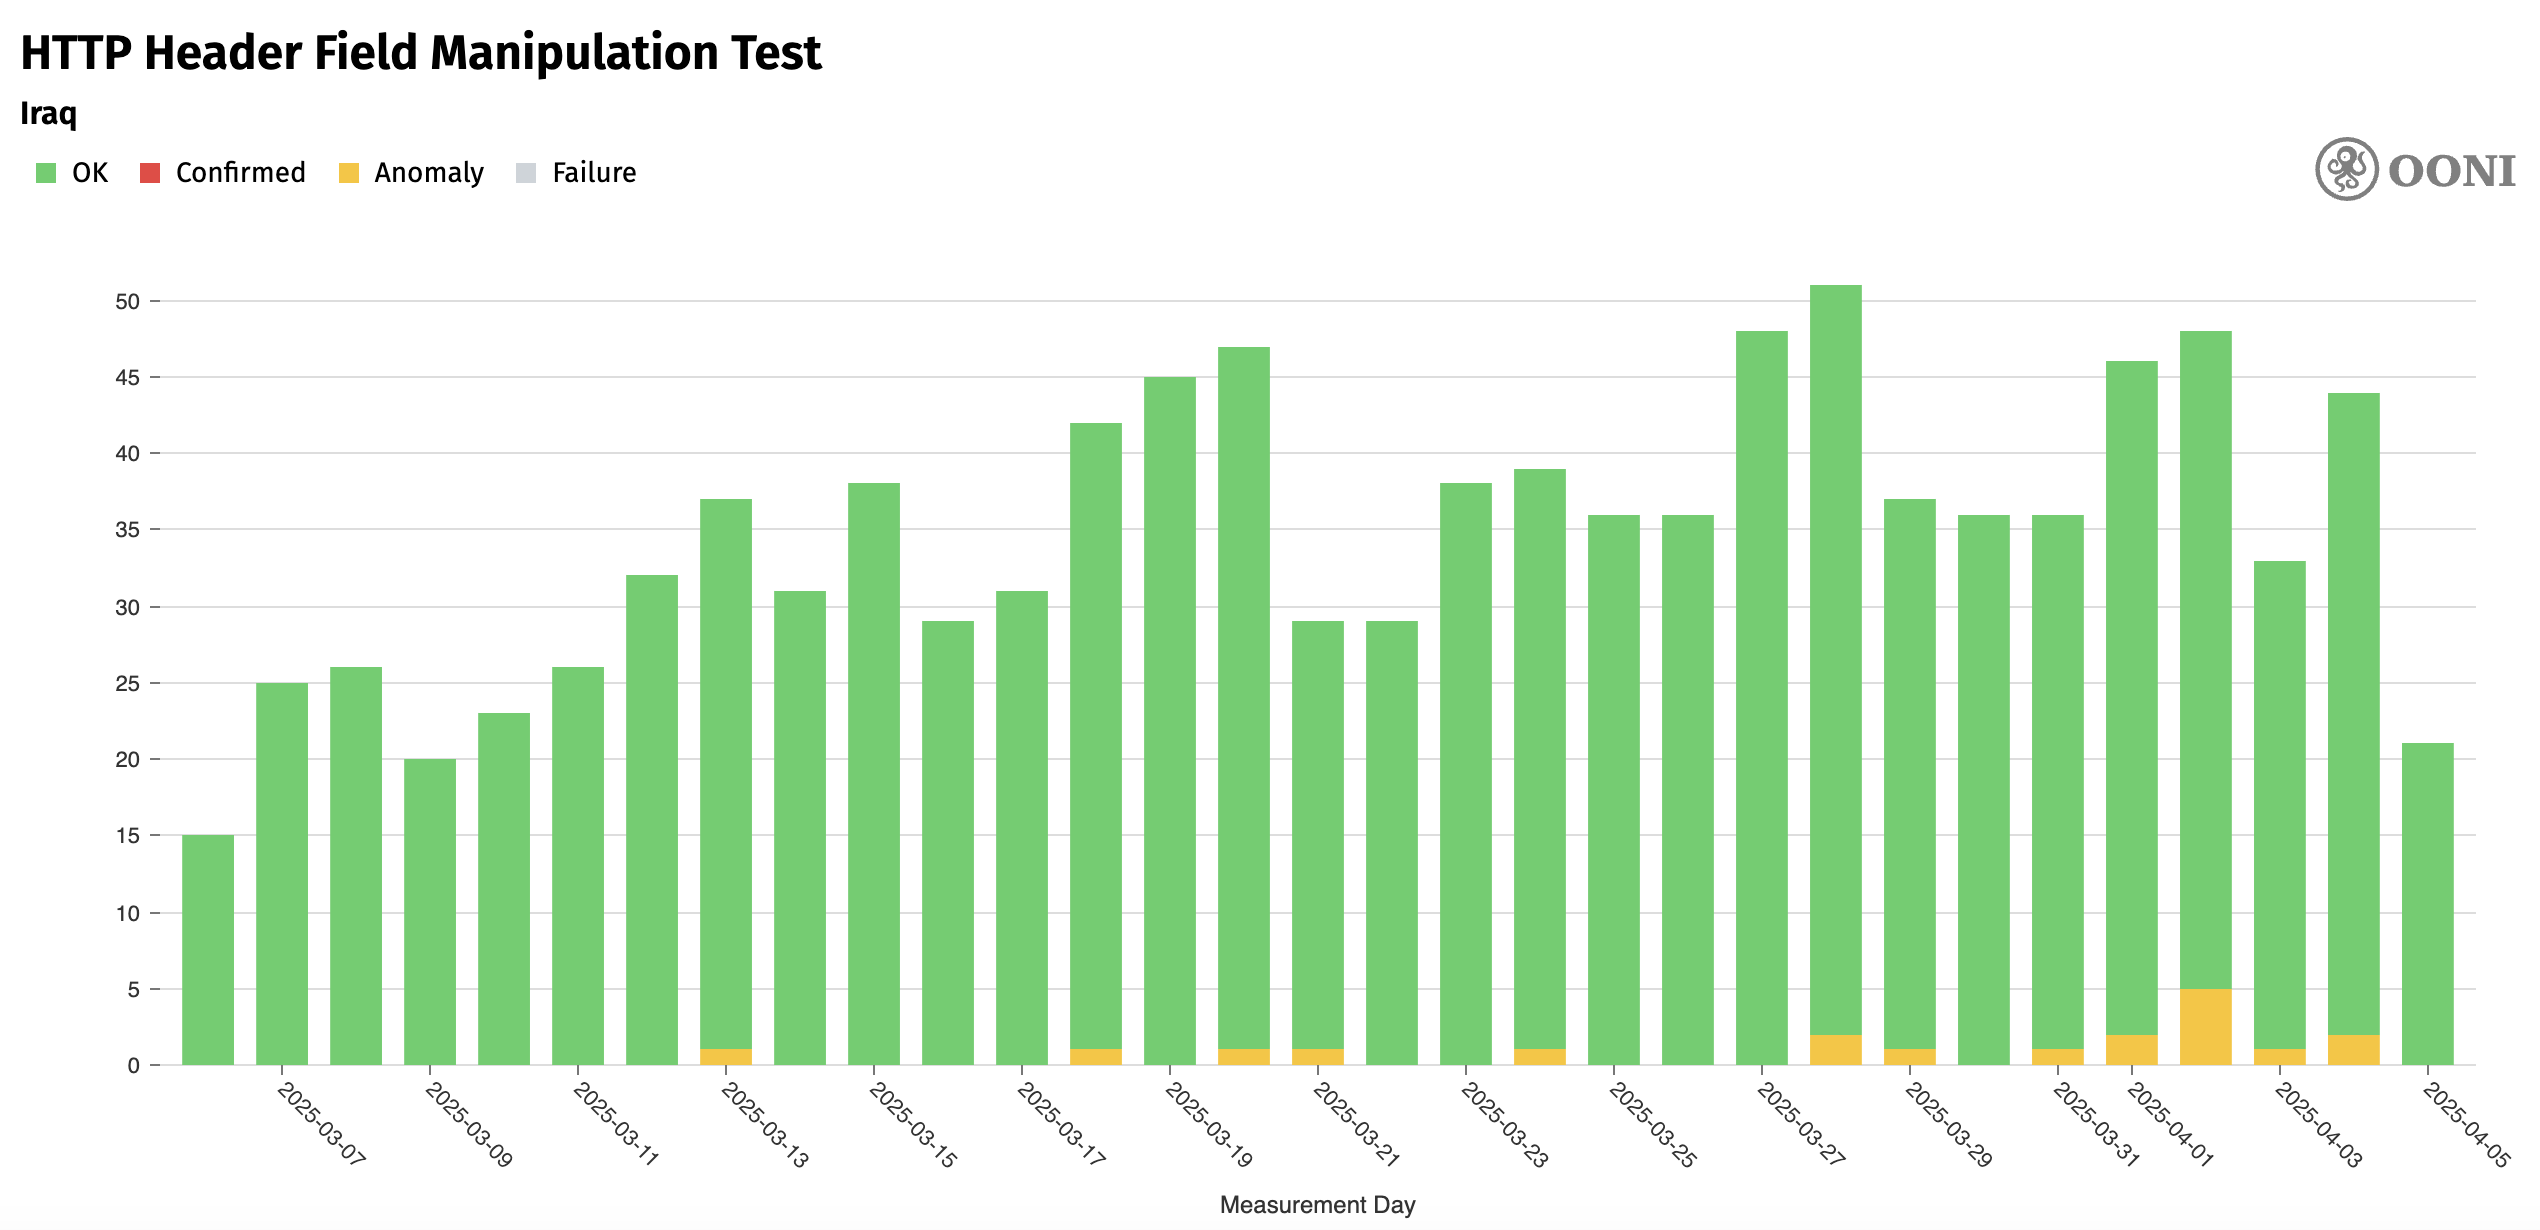
\includegraphics[width=\textwidth]{Griff/TCD SCSS CAPSTONE/Results/IraqMiddleboxHTTPManipulation.png}
%    \caption{Iraq Middlebox HTTP Header Field Manipulation Test: March 6, 2025 -- April 6, 2025}
%    \label{fig:iraq-middlebox-HTTP-manipulation}
%\end{figure}

\textit{Note: All CSV files gathered from the public OONI database can be found on the public GitHub for this work; see Appendix A1.2.}


\section{Comparative Analysis: Ireland v. Iraq}

The combined results of OONI probe testing and public OONI data reveal differences in censorship between Ireland and Iraq. While both countries implement content restrictions and other blocks, there are significant differences in the scale and motivations behind these blocks.

\subsubsection{Website Accessability}
\label{sec:Website-Accessability-Analysis}

The manually run web connectivity test yielded unexpected results. The proportion of blocked websites in both countries was similar, with Ireland having a slight edge over Iraq. This was unexpected, but because these tests were run manually on only one or two networks in each country, these results may only give a partial view of the country's Internet censorship. The results become more expected when looking at the publicly available OONI data. In the 30 days, Iraq blocked significantly more websites than Ireland and at a higher rate. Of the 3703 websites tested in Iraq, 262 had anomalies (7\% blocking rate), while of the 1695 websites tested in Ireland, only 43 had anomalies (2.5\% blocking rate). Looking at the figures, it is clear that Iraq blocks more content and on a more consistent basis than Ireland.

The blocking rates of websites by category reveal more expected results. Ireland blocked significantly more Piracy / Streaming / File Sharing websites outside of uncategorized websites than Iraq, which aligns with Ireland's court-mandated approach to censorship. Conversely, Iraq blocked a wider range of content by category, with a significant blocking rate of religious websites (75\%).

TCP/IP blocking was the top blocking method in both countries, indicating simple censorship mechanisms. Ireland, however, had a significantly higher rate of DNS blocking, which is likely due to its approach to targeted website blocking and EU compliance.

\subsubsection{Circumvention Tools}

The accessibility of Tor and Psiphon was essentially the same in Ireland and Iraq, with a few exceptions. Tor was widely accessible in both countries, indicating that Ireland and Iraq have no significant mechanisms to block this tool. If they do, there is no evidence that it is effective. There is evidence that Psiphon is blocked on specific ASNs in both countries, with public OONI data backing this up. In Ireland, Psiphon is blocked on HEAnet CLG (AS1213), as indicated by manually tested and public data. Over the same 30-day period, Ireland and Iraq blocked Psiphon 12.1\% of the time. As a result, there is little evidence of systemic efforts to block access to Psiphon, similar to Tor.

\subsubsection{Instant Messaging Platforms}

In Ireland, there is no evidence that instant messaging services are blocked meaningfully. This is in line with Ireland's stance on censorship and was expected. In Iraq, however, there is evidence that instant messaging services are blocked in some areas, but according to public OONI data, they are widely accessible. Some ASNs had implemented blocks on all four services tested to some capacity, indicating regional blocking in response to specific events. This is aligned with Iraq's more reactionary censoring practice.

\subsubsection{Presence of Middleboxes}

The use of Middleboxes in Ireland was almost non-existent, as there were only two anomalies over the 30-day period. These were likely false positives. This data indicates that Ireland does not implement TLS or SNI-based filtering systematically or widely. By contrast, Iraq showed significant evidence of Middleboxes being present. AS198589 showed significant signs of Middleboxes being present, and other ASNs have significant anomalies. This indicates that Iraq may implement TLS or SNI-based filtering in some areas of the country, which makes sense as we know that much of Iraq's current censorship efforts are decentralized. 

\subsection{Summary of Comparative Observations}

\begin{table}[H]
\centering
\caption{Comparative Summary of Internet Censorship: Ireland vs. Iraq}
\begin{tabular}{lcc}
\toprule
\textbf{Metric} & \textbf{Ireland} & \textbf{Iraq} \\
\midrule
Block Rate (OONI) & 2.5\% & 7\% \\
Blocking Methods & TCP/IP, DNS & TCP/IP, DNS, SNI \\
Tool Blocking & Rare, selective & Targeted, ASN-specific \\
Messaging Blocking & Negligible & Present on some ASNs \\
Middleboxes Detected & Minimal & Present on some ASNs \\
Motivations & Legal, EU compliance & Political, cultural control \\
\bottomrule
\end{tabular}
\label{tab:comparison_summary}
\end{table}

These findings support the initial research, showing that Ireland and Iraq have different censorship approaches. Ireland maintains a limited, legal-centric censorship model that is transparent and aligned with most other Western nations. Iraq's approach, while less centralized, is more reactive and inconsistent, often tied to internal events. 

\subsection{Future Work}

During this work, it became clear that exporting detailed public OONI data for web connectivity tests would be difficult. This public data would have provided more detailed insights into the differences between Ireland and Iraq. Future research could gather this data using the OONI public API to build upon this work. Using this API would allow for the automated collection of web connectivity data in Ireland and Iraq, giving the writer a broader foundation for comparison. This data would include blocking types, website categories, and ASN information.

Incorporating this public OONI data would facilitate a more holistic analysis of each country, as manual testing is only limited to one geographical location. This work shows that OONI tests yield different results in different regions of both countries, so relying solely on manually collected web connectivity data only gives a partial view of a country's current internet censorship. 